\section{Non-Functional Requirements}
\label{sec:non-functional-requirements}\label{sec:nfr-traceability}
This section specifies verifiable performance, usability, accessibility, security,
privacy, reliability and offline-continuity properties for the functional baseline.

\paragraph{Status and verification.}\label{sec:nfr-targets}
The working-specification status in Section~\ref{sec:document-status} applies.
Existing policies are 15-day offline authorisation, separate 30-day cache inactivity
cleanup and the 10~MB upload limit. Authentication, recovery, availability,
performance and usability targets have now been approved for this specification.
Concrete mechanisms, deployment resources and execution evidence remain team tasks under
the residual validations in Section~\ref{sec:validation-pending}. Verification requires configuration and
recorded evidence.

Use \identifier{PERF-01}--\identifier{PERF-08}, \identifier{USA-01}--\identifier{USA-09},
\identifier{SEC-01}--SEC-11, \identifier{PRV-01}--PRV-07, \identifier{REL-01}--REL-08 and \identifier{AOC-01}--AOC-06 with lettered
criteria, for example \identifier{SEC-03(d)}. Each requirement's \emph{Related}
links identify its functional applicability; Section~\ref{sec:nfr-validation}
provides planned verification scenarios. Record approved configuration, stimulus,
environment, expected response and observed measure when executing a quality
scenario.

\subsection{Performance}\label{sec:nfr-performance}
All workloads, sampling plans and timing limits in this subsection are approved
working-specification acceptance targets under \decisionref{Q-NFR-07}; they are not
measured capacity, executed results or an infrastructure procurement commitment. Correct results and accurate save states remain required:
speed does not compensate for lost work, duplicate effects or incorrect totals.

\subsubsection{Reference Conditions}\label{sec:nfr-performance-reference}
Use synthetic data in one owner workspace: 20 properties, 40 optional parcels,
10 campaigns, 100 workers, 180 working dates, 5,000 daily attendance decisions,
10,000 actual periods, 2,000 deliveries, 2,000 tickets and 2,000 analyses. These are
test fixtures, not capacity limits. Validate campaign coverage and dates, unique
business/day attendance, separate area assignments and at-most-one ticket/analysis.
Use client-validated weight/yield meanings; do not settle open source questions
through invented fixture calculations. The central history is not assumed to be
entirely prepared offline: record each offline scenario's authorised local subset.

Exercise five simultaneous authenticated sessions. Use a representative mid-range
phone with at least 4 GB RAM, a representative tablet and a desktop browser for the required computer layout. Record exact hardware, operating system, browser, server resources, build
and dataset versions. The reference online profile is at least 10 Mbps download,
2 Mbps upload and at most 150 ms round-trip latency. Document cache state and
separate cached/uncached runs; initial installation, login and preparation are online
prerequisites. Disable the network only after successful scoped preparation.

For \identifier{PERF-01}--\identifier{PERF-07}, collect at least 30 independent samples
per applicable device, operation and mode; at least 95\% must meet the approved
limit. Measure from the initiating action to usable content, completed calculation
or accurate save state, including applicable rendering and network time. Record
errors as failures. \identifier{PERF-08} instead uses ten complete reconnect cycles;
its benchmark is defined in \identifier{PERF-08}.

The upload policy remains \hyperref[br:044]{\identifier{BR-044}}. Reference
file sizes do not reduce that limit. Worker-document generation under
\hyperref[fr:063]{\identifier{FR-063}} is included. The selected Spanish inventory appears in Table~\ref{tab:source-forms}; technical rendering/field checks and a representative generation performance fixture are team verification tasks under \decisionref{Q-DOC-01} and
\decisionref{Q-NFR-07}.

\Needspace{8\baselineskip}
\subsubsection{Performance Requirements}
\Needspace{7\baselineskip}
\nfrheading{\identifier{PERF-01} --- Application and property access}\label{nfr:PERF-01}
Authorised home and property views shall become usable promptly online and within prepared offline scope.

\textit{Rationale:} Field navigation must not wait for unavailable central services.

\textit{Related:} \hyperref[fr:002]{\identifier{FR-002}}, \hyperref[fr:011]{\identifier{FR-011}}, \hyperref[fr:015]{\identifier{FR-015}}, \hyperref[fr:023]{\identifier{FR-023}}.
\begin{enumerate}[label=(\alph*),leftmargin=*,itemsep=1pt,topsep=3pt]
\item Target: usable authorised home and property list within 3 seconds under the reference profile; apply the same limit to prepared offline reopening.
\item Measure online opening and prepared reopening separately, distinguishing cached and uncached runs. Expose unavailable local detail without blocking unrelated navigation.
\end{enumerate}

\Needspace{7\baselineskip}
\nfrheading{\identifier{PERF-02} --- Worker and schedule consultation}\label{nfr:PERF-02}
Worker searches, prepared profiles and schedule changes shall provide timely usable results.

\textit{Rationale:} Daily consultation should remain practical with the reference workforce and history.

\textit{Related:} \hyperref[fr:023]{\identifier{FR-023}}, \hyperref[fr:028]{\identifier{FR-028}}.
\begin{enumerate}[label=(\alph*),leftmargin=*,itemsep=1pt,topsep=3pt]
\item Target: each worker search, prepared-profile opening and daily/worker/weekly view change completes within 2 seconds.
\item Test filters, matching and empty results, and unavailable prepared dates. Offline timing covers only authorised available scope; a retrieval failure is not a successful empty query.
\end{enumerate}

\Needspace{7\baselineskip}
\nfrheading{\identifier{PERF-03} --- Working-time previews and validation feedback}\label{nfr:PERF-03}
Supported local work calculations and validation feedback shall respond promptly to input changes.

\textit{Rationale:} Group entry needs immediate feedback before explicit confirmation.

\textit{Related:} \hyperref[fr:026]{\identifier{FR-026}}, \hyperref[fr:031]{\identifier{FR-031}}, \hyperref[fr:032]{\identifier{FR-032}}, \hyperref[fr:033]{\identifier{FR-033}}.
\begin{enumerate}[label=(\alph*),leftmargin=*,itemsep=1pt,topsep=3pt]
\item Target: update supported previews and validation feedback within 1 second for a 25-worker group with up to 100 periods.
\item Use the counted-time rules in Section~\ref{sec:counted-working-time}, including overnight work and worker-specific breaks and rejected overlapping-break proposals. Missing tasks/hours remain incomplete, not invented durations or counted unclassified periods.
\item Compare local checks with central validation on the same fixtures. Local feedback neither guarantees acceptance nor settles pending source-weight or yield interpretations.
\end{enumerate}

\Needspace{7\baselineskip}
\nfrheading{\identifier{PERF-04} --- Local saving and connected acknowledgement}\label{nfr:PERF-04}
Work submissions shall provide timely and distinct local-save and central-acceptance feedback.

\textit{Rationale:} A quick interface response must reflect the actual persistence outcome.

\textit{Related:} \hyperref[fr:029]{\identifier{FR-029}}, \hyperref[fr:034]{\identifier{FR-034}}, \hyperref[fr:037]{\identifier{FR-037}}.
\begin{enumerate}[label=(\alph*),leftmargin=*,itemsep=1pt,topsep=3pt]
\item For 25 workers with up to 100 periods and 25 breaks, the local-save target is 3 seconds from submission to durable local confirmation.
\item For a valid online submission under the reference profile, the server-acknowledgement target is 3 seconds from submission. Record it separately from local persistence.
\item Interrupt transmission before and after central commit/acknowledgement. Report the actual or uncertain outcome; a timeout proves neither rejection nor acceptance.
\end{enumerate}

\Needspace{7\baselineskip}
\nfrheading{\identifier{PERF-05} --- Campaign indicators and source refresh}\label{nfr:PERF-05}
Eligible indicators and their supported filters shall load and refresh promptly after relevant changes.

\textit{Rationale:} Campaign review depends on current, correctly scoped source contributions.

\textit{Related:} \hyperref[fr:055]{\identifier{FR-055}}, \hyperref[fr:056]{\identifier{FR-056}}, \hyperref[fr:058]{\identifier{FR-058}}, \hyperref[fr:060]{\identifier{FR-060}}, \hyperref[fr:061]{\identifier{FR-061}}.
\begin{enumerate}[label=(\alph*),leftmargin=*,itemsep=1pt,topsep=3pt]
\item Target: campaign indicators and applicable property/parcel filters become usable within 4 seconds.
\item Refresh affected visible results within 4 seconds after that client receives an accepted change or durably saves a supported local proposal; do not imply instant delivery to disconnected devices.
\item Verify restricted scope, late source information after closure, mixed-load allocation and Delivered-only eligibility. Keep accepted and local provisional contributions distinct.
\end{enumerate}

\Needspace{7\baselineskip}
\nfrheading{\identifier{PERF-06} --- Prepared and online file opening}\label{nfr:PERF-06}
Authorised prepared and online documents shall open within a measured reference-file budget.

\textit{Rationale:} Field consultation depends on both file readiness and usable viewing.

\textit{Related:} \hyperref[fr:038]{\identifier{FR-038}}, \hyperref[fr:039]{\identifier{FR-039}}, \hyperref[fr:040]{\identifier{FR-040}}, \hyperref[fr:045]{\identifier{FR-045}}, \hyperref[fr:049]{\identifier{FR-049}}, \hyperref[fr:051]{\identifier{FR-051}}.
\begin{enumerate}[label=(\alph*),leftmargin=*,itemsep=1pt,topsep=3pt]
\item For a prepared authorised PDF/JPG/PNG reference file up to 2 MB, opening limits are 2 seconds offline and 10 seconds online.
\item Test current insurance and explicitly prepared signing documents; record larger-file performance separately. The reference size is not an upload limit: \identifier{BR-044} still applies to worker documents and source evidence.
\item Missing local files, denied access and failed transfers produce truthful guidance rather than a successful-open result.
\end{enumerate}

\Needspace{7\baselineskip}
\nfrheading{\identifier{PERF-07} --- Campaign PDF snapshot export}\label{nfr:PERF-07}
A campaign indicator snapshot shall be produced promptly from available authorised information.

\textit{Rationale:} Export must preserve the meaning and limitations of the visible campaign results.

\textit{Related:} \hyperref[fr:059]{\identifier{FR-059}}, \hyperref[fr:060]{\identifier{FR-060}}, \hyperref[fr:062]{\identifier{FR-062}}.
\begin{enumerate}[label=(\alph*),leftmargin=*,itemsep=1pt,topsep=3pt]
\item Target: a snapshot of up to ten pages is ready to open or download within 10 seconds under the applicable reference mode.
\item Inspect online and offline scope, generation time, completeness, freshness and pending labels. Include prepared monetary content only with its financial grant; offline finance is not categorically excluded.
\item This benchmark covers campaign snapshots, not template-based worker-document generation. \identifier{FR-063} remains included; its representative templates and performance fixture require separate review.
\end{enumerate}

\Needspace{7\baselineskip}
\nfrheading{\identifier{PERF-08} --- Reconnection throughput}\label{nfr:PERF-08}
A valid prepared structured-operation batch shall synchronise within an agreed reconnection budget.

\textit{Rationale:} Reconnection must recover field work without duplicate effects or hidden failures.

\textit{Related:} \hyperref[fr:004]{\identifier{FR-004}}, \hyperref[fr:029]{\identifier{FR-029}}, \hyperref[fr:034]{\identifier{FR-034}}, \hyperref[fr:037]{\identifier{FR-037}}, \hyperref[fr:048]{\identifier{FR-048}}.
\begin{enumerate}[label=(\alph*),leftmargin=*,itemsep=1pt,topsep=3pt]
\item Accept 100 valid structured operations totalling at most 1~MB within 60 seconds, excluding files. Start timing after connectivity and current authority validation complete; record access-validation time separately.
\item All ten reference reconnect cycles must meet the budget, preserving dependency order and one business effect per operation. Count only valid centrally accepted operations as complete.
\item Exclude file transfers from this benchmark; define the operation unit, dependency mix and payload profile before testing. Test denied authority, conflicts, business-rule failures and attachment recovery separately.
\end{enumerate}


\subsection{Usability and Accessibility}\label{sec:nfr-usability}
Use an approved sample of five representative participants, including an owner
representative, after at most 15 minutes of introductory guidance. Exercise the
included manager paths within their grants and worker participation without an
account. Record exact devices, tasks and facilitation under
\decisionref{Q-NFR-08}; record task completion, timing, assistance and errors.
This small sample supports a prototype review, not a population-wide claim.

The numerical success, timing and interface targets below are approved acceptance
targets, requiring observed validation evidence. Local confirmation, central acceptance, financial provisional/final
classification and unavailable data retain their meanings in Section~\ref{sec:sync-states}
and the business rules. Routine offline interaction follows
Section~\ref{sec:offline-interaction}.

\Needspace{7\baselineskip}
\nfrheading{\identifier{USA-01} --- Role-appropriate navigation}\label{nfr:USA-01}
The owner and included managers shall find their permitted operational workflows through consistent navigation.

\textit{Rationale:} The owner is an operational user as well as a business reviewer.

\textit{Related:} \hyperref[fr:007]{\identifier{FR-007}}, \hyperref[fr:024]{\identifier{FR-024}}, \hyperref[fr:028]{\identifier{FR-028}}, \hyperref[fr:030]{\identifier{FR-030}}, \hyperref[fr:038]{\identifier{FR-038}}, \hyperref[fr:046]{\identifier{FR-046}}, \hyperref[fr:055]{\identifier{FR-055}}.
\begin{enumerate}[label=(\alph*),leftmargin=*,itemsep=1pt,topsep=3pt]
\item Target: at least four of five participants find each applicable planning, work, document, delivery and indicator task within 30 seconds without facilitator help.
\item Exercise owner and authorised manager paths. Expose only permitted tasks; do not confine the owner to an executive-only dashboard.
\end{enumerate}

\Needspace{7\baselineskip}
\nfrheading{\identifier{USA-02} --- Efficient group and retrospective entry}\label{nfr:USA-02}
Group defaults and individual adjustments shall support practical end-of-day entry without continuous phone use.

\textit{Rationale:} Recorded actual work may differ from planning and need retrospective confirmation.

\textit{Related:} \hyperref[fr:024]{\identifier{FR-024}}, \hyperref[fr:031]{\identifier{FR-031}}, \hyperref[fr:032]{\identifier{FR-032}}, \hyperref[fr:035]{\identifier{FR-035}}, \hyperref[fr:047]{\identifier{FR-047}}, \hyperref[fr:049]{\identifier{FR-049}}.
\begin{enumerate}[label=(\alph*),leftmargin=*,itemsep=1pt,topsep=3pt]
\item Target: at least four of five participants complete the reference task in less than 10 minutes without facilitator help, from opening the workflow to local confirmation.
\item Use 25 prepared workers, two eligible work areas, machinery/general tasks, one worker-specific break, one individual adjustment and two completed deliveries with supplied ticket data. Confirm valid campaign-start context before entry.
\item Check required tasks, attendance, times and individual differences. Measure synchronisation separately; successful local entry is not central acceptance.
\end{enumerate}

\Needspace{7\baselineskip}
\nfrheading{\identifier{USA-03} --- Planning, attendance and actual-work clarity}\label{nfr:USA-03}
Users shall distinguish planned work, daily presence, campaign-area participation, confirmed periods and synchronisation.

\textit{Rationale:} Profile capability and incomplete records must not be mistaken for actual counted work.

\textit{Related:} \hyperref[fr:020]{\identifier{FR-020}}, \hyperref[fr:028]{\identifier{FR-028}}, \hyperref[fr:030]{\identifier{FR-030}}, \hyperref[fr:031]{\identifier{FR-031}}, \hyperref[fr:033]{\identifier{FR-033}}.
\begin{enumerate}[label=(\alph*),leftmargin=*,itemsep=1pt,topsep=3pt]
\item Show missing tasks/hours and awaiting attendance explicitly. Machinery capability does not establish the actual task; overnight periods show both dates and their start-based working date.
\item Target: at least four of five participants correctly interpret each reference example, including a worker in two areas and an incomplete assignment without a task. An unclassified period is not a valid confirmed complete period.
\end{enumerate}

\Needspace{7\baselineskip}
\nfrheading{\identifier{USA-04} --- Insurance and version clarity}\label{nfr:USA-04}
Document views shall distinguish version currency, withdrawal, recorded expiry and worker-specific signing information.

\textit{Rationale:} A current file is not necessarily valid, signed or prepared on the device.

\textit{Related:} \hyperref[fr:038]{\identifier{FR-038}}, \hyperref[fr:039]{\identifier{FR-039}}, \hyperref[fr:041]{\identifier{FR-041}}, \hyperref[fr:044]{\identifier{FR-044}}.
\begin{enumerate}[label=(\alph*),leftmargin=*,itemsep=1pt,topsep=3pt]
\item Present current source, withdrawal and signing status separately; explain that replaced sources are deleted and have no history view; missing expiry is unconfirmed, not verified coverage.
\item Ask participants to locate prepared insurance and interpret expired, unconfirmed, withdrawn and unsigned examples. Explain missing local files/preparation failures without implying missing business records.
\end{enumerate}

\Needspace{7\baselineskip}
\nfrheading{\identifier{USA-05} --- Reviewable signing interaction}\label{nfr:USA-05}
Signing shall identify the worker and exact version and require deliberate review and confirmation.

\textit{Rationale:} Signing speed must not limit document reading or trigger duplicate signatures.

\textit{Related:} \hyperref[fr:042]{\identifier{FR-042}}, \hyperref[fr:043]{\identifier{FR-043}}, \hyperref[fr:044]{\identifier{FR-044}}, \hyperref[fr:045]{\identifier{FR-045}}.
\begin{enumerate}[label=(\alph*),leftmargin=*,itemsep=1pt,topsep=3pt]
\item Show worker/version, permit drawing, clearing/redrawing or cancellation before explicit confirmation, and reject empty drawings.
\item Target: at least four of five participants complete the interface interaction within 2 minutes after document review. Record reading time separately without a reading-time limit.
\item Test prepared online/offline and individual-document generation/signing paths. Check an uncertain prior submission before requesting another drawing; preserve worker/version-specific results.
\end{enumerate}

\Needspace{7\baselineskip}
\nfrheading{\identifier{USA-06} --- Terminology, sources and summary meaning}\label{nfr:USA-06}
Operational labels and summaries shall make their source, scope, units and uncertainty understandable.

\textit{Rationale:} Readable totals must not imply unsupported prices, payments or allocations.

\textit{Related:} \hyperref[fr:049]{\identifier{FR-049}}, \hyperref[fr:051]{\identifier{FR-051}}, \hyperref[fr:053]{\identifier{FR-053}}, \hyperref[fr:055]{\identifier{FR-055}}, \hyperref[fr:056]{\identifier{FR-056}}, \hyperref[fr:058]{\identifier{FR-058}}, \hyperref[fr:059]{\identifier{FR-059}}, \hyperref[fr:060]{\identifier{FR-060}}.
\begin{enumerate}[label=(\alph*),leftmargin=*,itemsep=1pt,topsep=3pt]
\item Use English for the report, prototype and current operational interface; preserve Spanish wording in the four generated forms. Use DD/MM/YYYY, 24-hour times, decimal comma and two displayed decimal places for percentages/EUR amounts; preserve source precision for weights/areas under \decisionref{Q-NFR-08}. Use explicit units and unambiguous dates; distinguish property/parcel provenance, tree/ground/mixed collection and actual task.
\item Explain incomplete, unallocated and unavailable results separately from valid zero. Keep reported financial provisional/final status distinct from local pending acceptance.
\item Use unknown yield, mixed provenance and partial-authority examples. Participants identify scope/source meaning without assuming price calculation, payment or automatic area allocation.
\end{enumerate}

\Needspace{7\baselineskip}
\nfrheading{\identifier{USA-07} --- Outdoor touch interaction}\label{nfr:USA-07}
Core field controls shall support readable and deliberate touch interaction on the supported devices.

\textit{Rationale:} Outdoor conditions can make small controls and colour-only feedback difficult to use.

\textit{Related:} \hyperref[fr:028]{\identifier{FR-028}}, \hyperref[fr:030]{\identifier{FR-030}}, \hyperref[fr:031]{\identifier{FR-031}}, \hyperref[fr:038]{\identifier{FR-038}}, \hyperref[fr:042]{\identifier{FR-042}}, \hyperref[fr:046]{\identifier{FR-046}}, \hyperref[fr:049]{\identifier{FR-049}}.
\begin{enumerate}[label=(\alph*),leftmargin=*,itemsep=1pt,topsep=3pt]
\item Targets: primary touch controls at least 44 by 44 CSS pixels and text contrast at least 4.5:1. Space controls to reduce accidental activation and never encode meaning by colour alone.
\item Use suitable mobile numeric/time inputs. Measure controls/contrast and test representative field devices outdoors, recording sunlight and glove conditions rather than claiming universal hardware compatibility.
\end{enumerate}

\Needspace{7\baselineskip}
\nfrheading{\identifier{USA-08} --- Responsive forms and accessible controls}\label{nfr:USA-08}
Core forms, actions and feedback shall remain usable across the agreed viewport, zoom and input modes.

\textit{Rationale:} Phone, tablet and keyboard users need access to the same permitted actions.

\textit{Related:} \hyperref[fr:024]{\identifier{FR-024}}, \hyperref[fr:028]{\identifier{FR-028}}, \hyperref[fr:030]{\identifier{FR-030}}, \hyperref[fr:036]{\identifier{FR-036}}, \hyperref[fr:038]{\identifier{FR-038}}, \hyperref[fr:042]{\identifier{FR-042}}, \hyperref[fr:055]{\identifier{FR-055}}.
\begin{enumerate}[label=(\alph*),leftmargin=*,itemsep=1pt,topsep=3pt]
\item Targets: core forms and primary actions usable at 360 CSS pixels without horizontal scrolling, and controls/messages accessible at 200\% zoom. Document viewers may pan source pages while retaining usable controls.
\item Provide associated labels, keyboard operation and visible focus for web controls, including those around document review and drawing. Validate on the agreed phone/tablet and supported desktop browser matrix.
\item Record which screens and interactions were checked; these selected criteria alone do not establish full accessibility conformance.
\end{enumerate}

\Needspace{7\baselineskip}
\nfrheading{\identifier{USA-09} --- Recoverable errors and informed corrections}\label{nfr:USA-09}
Errors and confirmations shall preserve recoverable input and explain the consequences of the requested operation.

\textit{Rationale:} A failed or cancelled action must not destroy unrelated work.

\textit{Related:} \hyperref[fr:035]{\identifier{FR-035}}, \hyperref[fr:036]{\identifier{FR-036}}, \hyperref[fr:037]{\identifier{FR-037}}, \hyperref[fr:041]{\identifier{FR-041}}, \hyperref[fr:043]{\identifier{FR-043}}.
\begin{enumerate}[label=(\alph*),leftmargin=*,itemsep=1pt,topsep=3pt]
\item Identify invalid fields and required corrections while preserving unaffected input. Cancellation before confirmation preserves accepted records; destructive actions identify consequences and require confirmation.
\item Test interrupted saves/uploads and presence-to-absence removal. Distinguish permitted completion after closure from confirmed-work correction requiring reopening; never silently rewrite plans or unrelated records.
\end{enumerate}


\subsection{Security}
\label{sec:nfr-security}
The API revalidates current account, workspace, scope and operation authority.
Prepared local data may be stale or affected by later revocation; a device timestamp
does not establish prior permission or acceptance. Figure~\ref{fig:nfr-security-boundaries}
summarises the proposed control boundaries, not an implemented security result.
\begin{figure}[htbp]
\centering
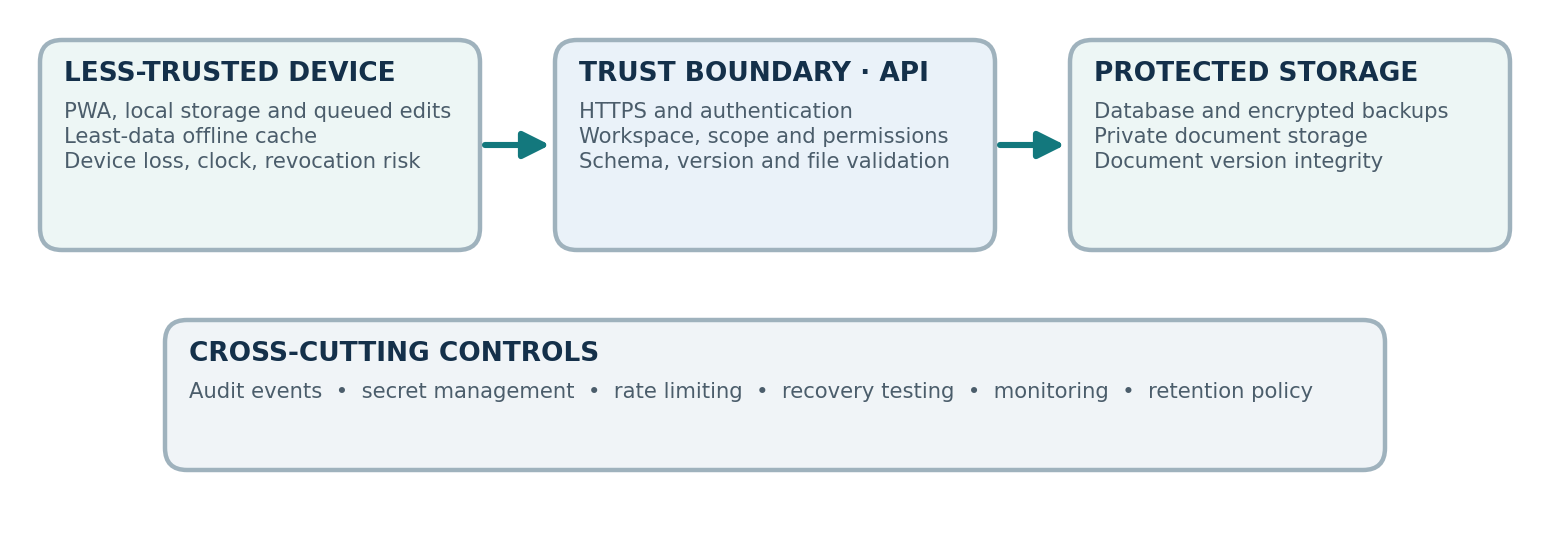
\includegraphics[width=\linewidth]{nfr-security-boundaries.png}
\caption{Proposed security boundaries and cross-cutting controls, adapted from the team's NFR contribution.}
\label{fig:nfr-security-boundaries}
\end{figure}

\Needspace{7\baselineskip}
\nfrheading{\identifier{SEC-01} --- Account authentication and password protection}\label{nfr:SEC-01}
The backend shall authenticate every application account using a unique, verified email identity and a password.

\textit{Rationale:} Protects the owner and included manager accounts against account takeover and enumeration.

\textit{Related:} \hyperref[fr:001]{\identifier{FR-001}}, \hyperref[fr:002]{\identifier{FR-002}}, \hyperref[fr:005]{\identifier{FR-005}}, \hyperref[fr:064]{\identifier{FR-064}}.
\begin{enumerate}[label=(\alph*),leftmargin=*,itemsep=1pt,topsep=3pt]
\item Only accounts with a verified email can access a business workspace; unverified accounts are refused.
\item Application-managed authentication uses established backend libraries and salted Argon2id password hashes; benchmark and record concrete cost parameters before deployment. Plaintext passwords are never stored or logged. A managed identity service is not the selected baseline.
\item Enforce at least 15 characters in the password-only flow and accept passphrases of at least 64 characters without silent truncation. Reject common/compromised passwords on registration, reset and change.
\item After five failed logins within 15 minutes, apply progressive throttling using account/source signals, without permanent attacker-triggered account lockout. Exact delay progression and recovery configuration require implementation review and tests.
\item Authentication failure responses do not disclose whether an email address is registered.
\end{enumerate}

\Needspace{7\baselineskip}
\nfrheading{\identifier{SEC-02} --- Online session lifecycle}\label{nfr:SEC-02}
Protected online requests shall use short-lived, revocable credentials.

\textit{Rationale:} Limits the exposure of stolen credentials and supports timely revocation.

\textit{Related:} \hyperref[fr:002]{\identifier{FR-002}}, \hyperref[fr:003]{\identifier{FR-003}}, \hyperref[fr:004]{\identifier{FR-004}}, \hyperref[fr:005]{\identifier{FR-005}}, \hyperref[fr:008]{\identifier{FR-008}}, \hyperref[fr:064]{\identifier{FR-064}}.
\begin{enumerate}[label=(\alph*),leftmargin=*,itemsep=1pt,topsep=3pt]
\item Online access credentials expire after 15 minutes; the server refuses expired credentials. Renewal is permitted only while the originating online session remains valid.
\item Renewable online sessions expire at most seven days after login, requiring authentication again; renewal does not extend that absolute limit. Implement revocation and rotation/replay protection. Cookie-based credentials use Secure, HttpOnly and an appropriate SameSite policy.
\item Logout revokes the applicable online session. Successful password reset or change invalidates existing online sessions. Membership revocation immediately denies that business online without deleting unrelated memberships.
\item An expired online session requires online renewal or authentication under its policy. It does not delete pending work or change the separate 15-day offline grant in \hyperref[nfr:AOC-02]{\identifier{AOC-02}}.
\end{enumerate}

\Needspace{7\baselineskip}
\nfrheading{\identifier{SEC-03} --- Workspace and operation-level authorisation}\label{nfr:SEC-03}
The server shall check authorisation on every protected read, write, export and file operation.

\textit{Rationale:} Preserves business isolation and independently granted consultation, entry and correction rights.

\textit{Related:} \hyperref[fr:002]{\identifier{FR-002}}, \hyperref[fr:004]{\identifier{FR-004}}, \hyperref[fr:007]{\identifier{FR-007}}, \hyperref[fr:008]{\identifier{FR-008}}, \hyperref[fr:023]{\identifier{FR-023}}, \hyperref[fr:038]{\identifier{FR-038}}, \hyperref[fr:053]{\identifier{FR-053}}; \hyperref[br:024]{\identifier{BR-024}}.
\begin{enumerate}[label=(\alph*),leftmargin=*,itemsep=1pt,topsep=3pt]
\item Each request validates account status and endpoint-specific authority. Technical provisioning requires the administrator system role; business operations require active workspace membership, responsibility scope and operation-specific grants. Administrator status alone grants no business-data/file authority.
\item A user-supplied identifier never establishes authority by itself.
\item Distinguish consultation, planning, entry, corrections, document association/modification, signing initiation and financial grants. Apply the included Field Manager defaults and mandatory scoped insurance access in Section~\ref{sec:permission-defaults}.
\item Supported financial actions may operate offline with the corresponding grants and prepared context; central acceptance revalidates them. Consultation/full-ticket access is disabled initially and requires an explicit owner grant within assigned scope; structured financial writes require additional grants.
\item Denied requests return a generic response that contains no protected data.
\end{enumerate}

\Needspace{7\baselineskip}
\nfrheading{\identifier{SEC-04} --- Encryption and private storage}\label{nfr:SEC-04}
Protected business data shall be encrypted in transit and in central storage; service credentials shall be protected and stored files private by default. Password storage follows \identifier{SEC-01} rather than reversible password encryption.

\textit{Rationale:} Protects employment, insurance and signing information across the device, API and storage boundaries.

\textit{Related:} \hyperref[fr:002]{\identifier{FR-002}}, \hyperref[fr:038]{\identifier{FR-038}}, \hyperref[fr:039]{\identifier{FR-039}}, \hyperref[fr:040]{\identifier{FR-040}}, \hyperref[fr:042]{\identifier{FR-042}}.
\begin{enumerate}[label=(\alph*),leftmargin=*,itemsep=1pt,topsep=3pt]
\item Production requests use HTTPS and a reviewed TLS/HSTS configuration. Plain HTTP is redirected or refused before protected content or credentials are served. The minimum supported protocol and deployment settings are reviewed under \decisionref{Q-TECH-01}.
\item Encrypt the central database, backups and private file storage at rest, with controlled key access and rotation. The hosting/key-management implementation is selected and verified during architecture review; this does not settle local-device protection under \decisionref{Q-DOC-07}.
\item Document storage is private by default; protected files are served only after API authorisation, using short-lived scoped retrieval links where applicable.
\item The central database is not directly reachable from the public internet.
\end{enumerate}

\Needspace{7\baselineskip}
\nfrheading{\identifier{SEC-05} --- Secure API, PWA and file validation}\label{nfr:SEC-05}
The backend shall validate every input and uploaded file independently of the PWA.

\textit{Rationale:} Prevents malicious requests, script injection and unsafe file handling; client-side validation does not replace server-side validation.

\textit{Related:} \hyperref[fr:001]{\identifier{FR-001}}, \hyperref[fr:038]{\identifier{FR-038}}, \hyperref[fr:040]{\identifier{FR-040}}, \hyperref[fr:045]{\identifier{FR-045}}, \hyperref[fr:049]{\identifier{FR-049}}, \hyperref[fr:051]{\identifier{FR-051}}, \hyperref[fr:053]{\identifier{FR-053}}, \hyperref[fr:063]{\identifier{FR-063}}, \hyperref[fr:064]{\identifier{FR-064}}.
\begin{enumerate}[label=(\alph*),leftmargin=*,itemsep=1pt,topsep=3pt]
\item Types, identifiers, relationships and file sizes are validated on the server, including references across business workspaces.
\item Use parameterised database access, context-appropriate output encoding, restrictive CORS and a deployable Content Security Policy. Cookie-authenticated state changes also require effective CSRF protection; CORS alone is not an authorisation or CSRF control.
\item Worker uploads accept PDF, JPG and PNG within the 10~MB (10,000,000-byte) per-file limit in \hyperref[br:044]{\identifier{BR-044}}. Validate content, size and safe file handling server-side, not only the extension. The team tests the 10,000,000-byte boundary and representative files under \decisionref{Q-DOC-06}; JPEG is accepted as the JPG image format.
\item Ticket, analysis and valuation evidence uses the same approved formats and 10~MB limit. Complete source files may be prepared offline with their consultation grants; monetary content neither forces classification/redaction nor prohibits upload under the applicable entry grant. Successful attachment replacement deletes its old file without history under \decisionref{Q-AT-02}; failed transfers preserve the old file and remain recoverable.
\item Scan application and bundled dependencies for known vulnerabilities in the delivery pipeline, triage findings and record remediation or explicit risk acceptance before release. A successful scan is not a claim of absence of vulnerabilities.
\end{enumerate}

\Needspace{7\baselineskip}
\nfrheading{\identifier{SEC-06} --- Secrets and deployment identities}\label{nfr:SEC-06}
Production credentials shall be kept out of source control and PWA assets, and every pipeline and service shall use least-privilege identities.

\textit{Rationale:} Prevents compromise through repository leakage or excessive pipeline privileges.

\textit{Related:} \hyperref[fr:001]{\identifier{FR-001}}, \hyperref[fr:005]{\identifier{FR-005}}, \hyperref[fr:040]{\identifier{FR-040}}.
\begin{enumerate}[label=(\alph*),leftmargin=*,itemsep=1pt,topsep=3pt]
\item Do not commit production service credentials or bundle database/email/storage secrets into the PWA. Device-local protection material, if used, follows the separate reviewed design under \decisionref{Q-DOC-07}.
\item Runtime services and delivery-pipeline jobs use separate identities with least privilege.
\item Keep production secrets in an access-controlled secrets mechanism with documented rotation and access review. Provider/tool selection remains an implementation decision.
\end{enumerate}

\Needspace{7\baselineskip}
\nfrheading{\identifier{SEC-07} --- Security-event audit logging}\label{nfr:SEC-07}
The server shall record security-relevant events.

\textit{Rationale:} Supports investigation and accountability while preserving the rule that ordinary business updates retain current values only (Section~\ref{sec:identity-current-values}).

\textit{Related:} \hyperref[fr:003]{\identifier{FR-003}}, \hyperref[fr:005]{\identifier{FR-005}}, \hyperref[fr:007]{\identifier{FR-007}}, \hyperref[fr:008]{\identifier{FR-008}}, \hyperref[fr:036]{\identifier{FR-036}}, \hyperref[fr:037]{\identifier{FR-037}}, \hyperref[fr:042]{\identifier{FR-042}}.
\begin{enumerate}[label=(\alph*),leftmargin=*,itemsep=1pt,topsep=3pt]
\item Each event records server timestamp, initiating account when known, workspace where applicable, action, minimal target identifier and outcome.
\item Mandatory server-observable categories: successful/failed authentication, logout, account recovery, membership and permission changes, restricted-document access requests handled by the API or controlled file service, signing acceptance, denied operations, revoked-access recovery decisions and security-relevant synchronisation conflicts. For document access, record the authorised retrieval/link-issuance decision or refusal; this does not prove that the user viewed the file.
\item Logs exclude passwords, raw tokens/full lifecycle links, document bodies, signature images, full official identification and raw monetary values; use minimal authorised identifiers.
\item Retain security events for 90 days from the server event, accessible only to authorised operations/investigation personnel. Purge thereafter, except justified incident preservation with a documented purpose and scope; test the configured schedule.
\item This requirement does not impose a permanent field-by-field history on ordinary corrections.
\item Opening a prepared file entirely offline is not logged in this version. Server preparation/retrieval/link issuance does not prove viewing. This coverage choice does not weaken file-access authorisation.
\end{enumerate}

\Needspace{7\baselineskip}
\nfrheading{\identifier{SEC-08} --- Document and signature integrity}\label{nfr:SEC-08}
Each accepted document version and each confirmed signature shall be tamper-evident and bound to the exact version signed.

\textit{Rationale:} Preserves integrity and provenance while respecting current-source replacement policy and withdrawal.

\textit{Related:} \hyperref[fr:038]{\identifier{FR-038}}, \hyperref[fr:041]{\identifier{FR-041}}, \hyperref[fr:042]{\identifier{FR-042}}, \hyperref[fr:043]{\identifier{FR-043}}, \hyperref[fr:044]{\identifier{FR-044}}, \hyperref[fr:045]{\identifier{FR-045}}; \hyperref[br:026]{\identifier{BR-026}}.
\begin{enumerate}[label=(\alph*),leftmargin=*,itemsep=1pt,topsep=3pt]
\item Each current accepted source has an immutable file identity and protected cryptographic digest. Verify source bytes against that digest. Validate the rendition against its own source/worker/signature associations; a derived PDF is not compared with the source digest. The team selects/tests the digest algorithm and metadata protection; a hash is not signer identification.
\item Bind a confirmed drawing to its worker, authorised initiator, exact source and confirmation time.
\item Never transfer a drawing or choice to another source/worker or overwrite signed bytes in place. A replacement needs its own worker review/signing.
\item Apply \identifier{BR-026}: only after successful replacement, delete the superseded source, signature and PDF, including signed contracts/externally declared signed uploads. Invalidate old-source signing and propagate received deletion to prepared copies. Temporary rejected-proposal recovery follows \decisionref{Q-DOC-04}, without a history browser.
\item Record server acceptance time separately from device confirmation time.
\item A drawn mark alone is not represented as a qualified electronic signature.
\end{enumerate}

\Needspace{7\baselineskip}
\nfrheading{\identifier{SEC-09} --- Verification, recovery and invitation tokens}\label{nfr:SEC-09}
Account-lifecycle links shall be single-use, short-lived and unpredictable.

\textit{Rationale:} Protects registration, recovery and invitation flows from replay, enumeration and unauthorised business membership.

\textit{Related:} \hyperref[fr:001]{\identifier{FR-001}}, \hyperref[fr:005]{\identifier{FR-005}}, \hyperref[fr:006]{\identifier{FR-006}}, \hyperref[fr:064]{\identifier{FR-064}}.
\begin{enumerate}[label=(\alph*),leftmargin=*,itemsep=1pt,topsep=3pt]
\item Owner-activation and email-verification links, including replacement-email verification, expire after 24 hours and are single-use. An unverified replacement cannot supersede the active email; a resend invalidates the preceding link.
\item Password-reset links expire after 30 minutes and are single-use. Resending invalidates the preceding link; invalid/expired/consumed links cannot change credentials.
\item Invitations expire after seven days and are single-use, bound to the intended verified email and business. Resending/cancelling invalidates superseded links without duplicate membership.
\item Generate token values unpredictably and store only a verification hash or equivalent protected verifier when persisted. Consume/invalidate lifecycle authorisations transactionally. Retries may report an already completed action without repeating activation, membership creation or credential changes.
\item A successful reset revokes existing online sessions without changing business ownership.
\end{enumerate}

\Needspace{7\baselineskip}
\nfrheading{\identifier{SEC-10} --- Abuse protection and rate limiting}\label{nfr:SEC-10}
The API shall limit request rates to protect availability and prevent automated abuse.

\textit{Rationale:} \hyperref[nfr:SEC-01]{\identifier{SEC-01}} throttles login attempts only; recovery, invitation, upload and email-triggering endpoints can also be abused.

\textit{Related:} \hyperref[fr:001]{\identifier{FR-001}}, \hyperref[fr:005]{\identifier{FR-005}}, \hyperref[fr:006]{\identifier{FR-006}}, \hyperref[fr:040]{\identifier{FR-040}}.
\begin{enumerate}[label=(\alph*),leftmargin=*,itemsep=1pt,topsep=3pt]
\item Use account/source/recipient-aware limits as applicable: unauthenticated operations cannot depend on an authenticated account key. Apply stricter reviewed controls to authentication, recovery, invitations, uploads and email-triggering requests.
\item Exceeded limits return a generic, retryable rejection and do not affect other accounts.
\item Resending verification, reset and invitation messages is limited per recipient address.
\item The approved login threshold is five failures within 15 minutes under SEC-01. Endpoint-specific recovery, resend, upload and invitation limits and progressive delays still require configuration review; verify recipient/account isolation before release.
\end{enumerate}

\Needspace{7\baselineskip}
\nfrheading{\identifier{SEC-11} --- Email delivery security}\label{nfr:SEC-11}
Verification, recovery and invitation messages shall be sent through an authenticated and monitored email delivery service.

\textit{Rationale:} Protects account activation, recovery, verified-email changes and invitations that depend on email delivery.

\textit{Related:} \hyperref[fr:001]{\identifier{FR-001}}, \hyperref[fr:005]{\identifier{FR-005}}, \hyperref[fr:006]{\identifier{FR-006}}, \hyperref[fr:064]{\identifier{FR-064}}.
\begin{enumerate}[label=(\alph*),leftmargin=*,itemsep=1pt,topsep=3pt]
\item The sending domain is authenticated with SPF, DKIM and DMARC.
\item Messages contain the intended lifecycle link and minimal account context, never passwords, worker data or protected documents.
\item A send failure preserves the pending account/invitation state without duplicate identities or memberships. Offer rate-limited resend, invalidating the preceding lifecycle link. Recovery acknowledgements remain generic regardless of registration status.
\item Record the provider, its processing role/terms, sending-domain configuration and any transfers in the processing inventory under \hyperref[nfr:PRV-05]{\identifier{PRV-05}}; provider selection remains under \decisionref{Q-NFR-05}.
\end{enumerate}

\paragraph{Email delivery operation.}
Only the backend calls the transactional email service using protected credentials.
Record technical send outcomes and provider failures without full links. Provider
acceptance does not prove inbox delivery or reading. Development/demo sending uses
controlled recipients or a test environment. Provider, authorised sender domain and
concrete configuration remain under \decisionref{Q-NFR-05}.

\paragraph{Technical references.}
Password and session controls are informed by the
\href{https://cheatsheetseries.owasp.org/cheatsheets/Authentication_Cheat_Sheet.html}{OWASP Authentication},
\href{https://cheatsheetseries.owasp.org/cheatsheets/Password_Storage_Cheat_Sheet.html}{Password Storage}
and \href{https://cheatsheetseries.owasp.org/cheatsheets/Session_Management_Cheat_Sheet.html}{Session Management}
guidance. These references do not approve project-specific numeric targets.

\paragraph{Administrator provisioning verification.}
Check administrator-only owner setup, single-client concurrency/idempotency,
expired/replayed activation, controlled resend and recipient-chosen password.
Unauthenticated users, owners and managers cannot call technical provisioning;
technical administrators cannot read agricultural records/files by system role alone.
Manager signup requires an intended valid owner invitation. Bootstrap credentials
are deployment-managed; passwords never enter provisioning messages or logs.

\subsection{Privacy}
\label{sec:nfr-privacy}
Protect account data and worker records, including required official identification,
insurance, employment documents, drawn signatures and examination-consent choices.
Clinical findings are outside this form workflow. Source member references and
official worker identifiers remain protected business data. The processing basis and
retention duties must be validated for the actual context; technical controls alone
do not establish GDPR compliance. \identifier{PRV-04} defines governance procedures without
silently adding account deletion or worker self-service to the functional scope.

\Needspace{7\baselineskip}
\nfrheading{\identifier{PRV-01} --- Personal-data minimisation and purpose limitation}\label{nfr:PRV-01}
The application shall collect and expose only the personal data needed for documented purposes.

\textit{Rationale:} Workers have no management accounts; owners and authorised managers process their records within a business workspace.

\textit{Related:} \hyperref[fr:020]{\identifier{FR-020}} to \hyperref[fr:023]{\identifier{FR-023}}, \hyperref[fr:038]{\identifier{FR-038}}, \hyperref[fr:039]{\identifier{FR-039}}, \hyperref[fr:053]{\identifier{FR-053}}.
\begin{enumerate}[label=(\alph*),leftmargin=*,itemsep=1pt,topsep=3pt]
\item Document the purpose and necessity of account/worker attributes, including the official type, country and number required by \hyperref[fr:020]{\identifier{FR-020}}. Required entry does not itself establish a lawful basis or require collection of a scanned copy.
\item Each cached dataset and exported report is limited to the authenticated user's authorised responsibilities.
\item Full document contents and unrelated personal identifiers are not copied into dashboards or technical logs.
\end{enumerate}

\Needspace{7\baselineskip}
\nfrheading{\identifier{PRV-02} --- Lawful processing and transparency}\label{nfr:PRV-02}
The responsible business shall document the lawful basis for worker data before real data are processed.

\textit{Rationale:} Consent may be inappropriate or insufficient in an employment relationship; compliance depends on purpose and legal context, not on hosting location.

\textit{Related:} \hyperref[fr:020]{\identifier{FR-020}} to \hyperref[fr:023]{\identifier{FR-023}}, \hyperref[fr:038]{\identifier{FR-038}} to \hyperref[fr:045]{\identifier{FR-045}}.
\begin{enumerate}[label=(\alph*),leftmargin=*,itemsep=1pt,topsep=3pt]
\item Before real worker data are used, the purposes, applicable lawful bases, privacy notice and processor responsibilities are documented for worker records, insurance, employment documents and signatures.
\item Do not assume that a generic GDPR consent signature authorises all employment processing. Validate the applicable basis by purpose, including any sensitive information in supplied documents; unresolved questions remain under \decisionref{Q-NFR-03}.
\item Academic demonstration and test environments use synthetic or appropriately anonymised data unless real-data processing has been authorised.
\end{enumerate}

\Needspace{7\baselineskip}
\nfrheading{\identifier{PRV-03} --- Protected local data and account isolation}\label{nfr:PRV-03}
Data held on the device shall be limited, isolated by account and protected after logout or revocation.

\textit{Rationale:} Prepared insurance and signing documents must be available offline while unsent work is safeguarded on logout.

\textit{Related:} \hyperref[fr:003]{\identifier{FR-003}}, \hyperref[fr:004]{\identifier{FR-004}}, \hyperref[fr:008]{\identifier{FR-008}}, \hyperref[fr:039]{\identifier{FR-039}}, \hyperref[fr:045]{\identifier{FR-045}}.
\begin{enumerate}[label=(\alph*),leftmargin=*,itemsep=1pt,topsep=3pt]
\item Prepared local datasets contain only authorised required context, with pending local records/dependencies created through supported offline operations stored separately from the accepted baseline.
\item Private data and pending operations are logically isolated by originating account and business workspace.
\item Logout immediately blocks workspace access and isolates retained information. Disposable accepted copies may be removed under the local policy; the 30-day inactivity cleanup in \hyperref[fr:003]{\identifier{FR-003}} removes only eligible accepted copies and never pending recovery dependencies.
\item Normal recovery requires the originating account and renewed authority. The separate revoked-manager owner-review procedure in \hyperref[fr:008]{\identifier{FR-008}}/\hyperref[nfr:REL-08]{\identifier{REL-08}} preserves original authorship without restoring normal access or exposing pending work to another account.
\item On reconnection, refresh authority before normal protected access/acceptance and apply authorised access/deletion changes. Preserve quarantined pending proposals and required recovery files under the separate recovery policy.
\item The system does not claim that a disconnected device can be remotely wiped immediately.
\item Encrypt device-held personal data, protected files and pending operations, isolated by origin account and business. Logout locks protected access while preserving recovery dependencies. Another account cannot read or submit them. Concrete encryption/key lifecycle and trusted-time mechanisms require a technical proof under \decisionref{Q-DOC-07}; browser-origin isolation or screen lock alone is insufficient.
\end{enumerate}

\Needspace{7\baselineskip}
\nfrheading{\identifier{PRV-04} --- Rights, retention and permitted erasure}\label{nfr:PRV-04}
Personal-data requests shall follow a documented authorised procedure that respects applicable rights, dependencies and validated retention duties.

\textit{Rationale:} Distinguishes rights handling from ordinary record deletion and avoids inventing unapproved self-service workflows.

\textit{Related:} \hyperref[fr:003]{\identifier{FR-003}}, \hyperref[fr:021]{\identifier{FR-021}} to \hyperref[fr:023]{\identifier{FR-023}}, \hyperref[fr:038]{\identifier{FR-038}}, \hyperref[fr:041]{\identifier{FR-041}}; \hyperref[br:026]{\identifier{BR-026}}.
\begin{enumerate}[label=(\alph*),leftmargin=*,itemsep=1pt,topsep=3pt]
\item Handle consultation, correction and erasure requests manually: the owner receives/follows the request; a designated technical responsible person intervenes when necessary and authorised. No dedicated request-management portal is included.
\item Record request identity, scope, authorisation, action and response through a controlled procedure. Assess dependencies and applicable processing duties; archival/inactivation is not itself erasure.
\item While a source exists, its contents and signing evidence remain immutable. Successful replacement deletes the previous source, signature and PDF for every category under \identifier{BR-026}, with no inherited signature or consultable history. A failed upload preserves the current source.
\item The agreed product rule keeps current documents until replacement rather than assigning an invented fixed number of years. Document the applicable purposes/notices and operating responsibilities before real-data use; deployment review does not assert completed legal validation.
\item Backup expiry and restore suppression follow \identifier{REL-04}. Apply retained deletion decisions before restoring normal access; do not claim immediate erasure from every backup or disconnected device.
\item Controlled account/data requests follow this manual procedure under \decisionref{Q-AA-07}; owner-facing business closure is excluded under \decisionref{Q-SCOPE-07}. Verified email changes under \identifier{FR-064} preserve account identity.
\end{enumerate}

\Needspace{7\baselineskip}
\nfrheading{\identifier{PRV-05} --- Processing location and breach response}\label{nfr:PRV-05}
Processing locations, providers and transfers shall be reviewed, and an operational personal-data incident procedure shall exist.

\textit{Rationale:} Hosting location alone does not establish GDPR compliance; organisational responsibilities and transfer arrangements also matter.

\textit{Related:} \hyperref[fr:001]{\identifier{FR-001}} to \hyperref[fr:008]{\identifier{FR-008}}, \hyperref[fr:038]{\identifier{FR-038}} to \hyperref[fr:045]{\identifier{FR-045}}.
\begin{enumerate}[label=(\alph*),leftmargin=*,itemsep=1pt,topsep=3pt]
\item Approve primary, backup, telemetry and support-processing locations before real-data deployment. EU-region hosting is the submitted preference for review under \decisionref{Q-NFR-03}, not a settled provider/deployment decision or a substitute for transfer assessment.
\item Processing terms and any international transfers are verified for infrastructure, support, telemetry and email-delivery providers.
\item An incident-response procedure identifies the controller contact, escalation route, containment and assessment steps.
\item Where GDPR Article 33 applies, the controller assesses notification without undue delay and, where feasible, within 72 hours after awareness, unless the breach is unlikely to risk individuals' rights and freedoms. Record the assessment and any reasons for delay; applicability and responsibility are validated under \decisionref{Q-NFR-03}.
\end{enumerate}

\Needspace{7\baselineskip}
\nfrheading{\identifier{PRV-06} --- Privacy-preserving telemetry}\label{nfr:PRV-06}
Logs, analytics and diagnostics shall not become an uncontrolled second copy of personal or financial data.

\textit{Rationale:} Observability must not expose protected documents or monetary values.

\textit{Related:} \hyperref[fr:038]{\identifier{FR-038}}, \hyperref[fr:045]{\identifier{FR-045}}, \hyperref[fr:053]{\identifier{FR-053}} to \hyperref[fr:062]{\identifier{FR-062}}.
\begin{enumerate}[label=(\alph*),leftmargin=*,itemsep=1pt,topsep=3pt]
\item Logs, analytics, error reports, queue diagnostics and deployment artefacts minimise personal data and exclude full official identification, document bodies and captured drawings. Operational identifiers are limited to the authorised diagnostic purpose.
\item Diagnostic records use record identifiers and minimal contextual metadata, with access control and a retention schedule.
\item Do not copy monetary values or protected document contents into technical diagnostics. This does not prohibit authorised financial business data, prepared offline consultation or PDF indicators under \hyperref[fr:053]{\identifier{FR-053}}, \hyperref[fr:060]{\identifier{FR-060}} and \hyperref[fr:062]{\identifier{FR-062}}.
\end{enumerate}

\Needspace{7\baselineskip}
\nfrheading{\identifier{PRV-07} --- Offline document retention and deletion propagation}\label{nfr:PRV-07}
Offline document preparation shall be selective, and deletions made centrally shall reach local copies.

\textit{Rationale:} Offline insurance and signing (\hyperref[fr:039]{\identifier{FR-039}}, \hyperref[fr:045]{\identifier{FR-045}}) must not expand personal-data exposure unnecessarily.

\textit{Related:} \hyperref[fr:038]{\identifier{FR-038}}, \hyperref[fr:039]{\identifier{FR-039}}, \hyperref[fr:041]{\identifier{FR-041}}, \hyperref[fr:042]{\identifier{FR-042}}, \hyperref[fr:045]{\identifier{FR-045}}.
\begin{enumerate}[label=(\alph*),leftmargin=*,itemsep=1pt,topsep=3pt]
\item Preparation covers current insurance versions for the prepared worker window and explicitly selected workers, and only specifically prepared versions for offline signing.
\item Contracts are never bulk-downloaded automatically.
\item Local file/reference metadata identifies the originating account and workspace, associated worker and version or authorised business target, access context and freshness and the document's single worker identity.
\item Apply received access, withdrawal and deletion changes to prepared copies. Remove superseded accepted source, signature and PDF copies after receiving replacement deletion; route ineligible pending signing to protected temporary recovery without resurrecting the old source. A withdrawn current source remains consultable until replacement but is ineligible for signing; replaced sources have no history view; exclusive local conflicts follow \decisionref{Q-DOC-04}.
\item Queued retries never recreate a deleted version.
\end{enumerate}

\paragraph{Regulatory reference.}
Validate the applicable duties against
\href{https://eur-lex.europa.eu/eli/reg/2016/679/oj}{Regulation (EU) 2016/679},
including purpose/minimisation, lawful basis, rights, processors, security,
notification and transfers. The incident-notification time in \identifier{PRV-05} is a conditional
legal requirement, not a proposed service-level target or a certification of compliance.

\subsection{Reliability and Recovery}
\label{sec:nfr-reliability}
These requirements protect accepted data and recoverable proposals during retries,
concurrent edits, interrupted transfers, upgrades and central recovery. The protocol
in Section~\ref{sec:offline-sync} supplies the interaction detail; the synchronisation
state definitions remain in Section~\ref{sec:sync-states}. Backup and service targets
are approved specification targets, not measured outcomes or provider guarantees.

\Needspace{7\baselineskip}
\nfrheading{\identifier{REL-01} --- Idempotent server processing}\label{nfr:REL-01}
Every mutating operation shall have the same business effect however many times it is submitted.

\textit{Rationale:} Retries after disconnection must not duplicate business records or signatures.

\textit{Related:} \hyperref[fr:001]{\identifier{FR-001}}, \hyperref[fr:003]{\identifier{FR-003}}, \hyperref[fr:006]{\identifier{FR-006}}, \hyperref[fr:029]{\identifier{FR-029}}, \hyperref[fr:041]{\identifier{FR-041}}, \hyperref[fr:043]{\identifier{FR-043}}, \hyperref[fr:048]{\identifier{FR-048}}.
\begin{enumerate}[label=(\alph*),leftmargin=*,itemsep=1pt,topsep=3pt]
\item Mutations carry stable operation\_id, origin, payload fingerprint and dependencies. Persist minimal outcomes for 90 days after processing. Identical retries have one effect; reused IDs with different content are refused. Expired-context submissions require reviewed recovery, never blind replay that could duplicate effects or recreate deleted records.
\item Creation of users, memberships, attendance, deliveries, document versions and signatures is protected against duplicate retries.
\item Related database changes and the idempotency outcome commit atomically. Transfers to object storage have a recoverable readiness/cleanup protocol; this is not a claim of one database/object-store transaction.
\end{enumerate}

\Needspace{7\baselineskip}
\nfrheading{\identifier{REL-02} --- Optimistic concurrency and conflict resolution}\label{nfr:REL-02}
Concurrent changes to shared records shall never be silently overwritten.

\textit{Rationale:} Supports informed user review of competing corrections.

\textit{Related:} \hyperref[fr:008]{\identifier{FR-008}}, \hyperref[fr:036]{\identifier{FR-036}}, \hyperref[fr:037]{\identifier{FR-037}}, \hyperref[fr:043]{\identifier{FR-043}}.
\begin{enumerate}[label=(\alph*),leftmargin=*,itemsep=1pt,topsep=3pt]
\item Every mutable shared record has a server-managed revision, and each update carries the client's base revision.
\item A version mismatch never overwrites accepted server state; the pending proposal is preserved.
\item The user sees accepted and proposed values side by side for authorised manual review.
\item Resubmission after review revalidates permissions, campaign state, dependencies and business rules.
\item Automatic last-write-wins is not used for any persisted business record.
\end{enumerate}

\Needspace{7\baselineskip}
\nfrheading{\identifier{REL-03} --- Cross-entity integrity and consistent calculations}\label{nfr:REL-03}
The API and the database shall enforce integrity rules, and server-side validation shall be authoritative even for data entered offline.

\textit{Rationale:} Ensures dashboard correctness and prevents cross-workspace or cross-campaign corruption.

\textit{Related:} \hyperref[fr:026]{\identifier{FR-026}} to \hyperref[fr:037]{\identifier{FR-037}}, \hyperref[fr:046]{\identifier{FR-046}} to \hyperref[fr:062]{\identifier{FR-062}}.
\begin{enumerate}[label=(\alph*),leftmargin=*,itemsep=1pt,topsep=3pt]
\item Foreign-key, uniqueness, business-scope and status-transition constraints are enforced.
\item Actual work periods are not double counted across assignments, campaigns or adjacent dates.
\item Delivery-based totals require Delivered, non-cancelled parents under \hyperref[br:038]{\identifier{BR-038}}. Pre-arrival source data awaits receipt confirmation. Ticket deductions are not applied twice; missing analyses are not treated as zero.
\item For one ticket, replacing a provisional amount with final retains one current valuation, never additive revisions. Separate provisional/final totals across different eligible tickets remain valid and do not imply payments.
\item Server-side validation prevails over local validation for data that originated offline.
\end{enumerate}

\Needspace{7\baselineskip}
\nfrheading{\identifier{REL-04} --- Central backup and tested recovery}\label{nfr:REL-04}
Central data shall be backed up and recoverable within stated targets.
The recovery point objective (RPO) bounds the recoverable data-loss window;
the recovery time objective (RTO) bounds the time to restore the agreed service
after a declared incident. Record both measurement boundaries in the rehearsal.

\textit{Rationale:} Makes central persistence recoverable; measurable objectives depend on an agreed deployment and a rehearsed restore procedure.

\textit{Related:} \hyperref[fr:003]{\identifier{FR-003}}, \hyperref[fr:038]{\identifier{FR-038}} to \hyperref[fr:045]{\identifier{FR-045}}, \hyperref[fr:046]{\identifier{FR-046}} to \hyperref[fr:062]{\identifier{FR-062}}; \hyperref[br:026]{\identifier{BR-026}}.
\begin{enumerate}[label=(\alph*),leftmargin=*,itemsep=1pt,topsep=3pt]
\item Automate encrypted central database and compatible file/evidence backups at least daily. Preserve database/file dependencies together, restrict access and alert on failed scheduled backups.
\item Retain central backups for at least 14 days. This is a recovery policy, not an employment or signed-document retention period or proof of immediate erasure from all backups.
\item Rehearse RPO at most 24 hours and RTO at most four hours against the agreed deployment/data restore scope. The accepted RPO permits up to 24 hours of central-data loss. These targets do not recover unsent records on a lost device.
\item Before restoring ordinary service, reapply retained authorised deletion/restriction and access decisions that postdate the backup. Retain recovery metadata independently long enough to enforce them; if it is insufficient, quarantine affected data rather than exposing erased/restricted records.
\item At least one representative restore rehearsal is performed before operational deployment, validating relationships and accessible retained document versions.
\end{enumerate}

\Needspace{7\baselineskip}
\nfrheading{\identifier{REL-05} --- Monitoring and incident response}\label{nfr:REL-05}
Failures shall be detected and reach a named team contact during the harvest period.

\textit{Rationale:} Field work may continue locally during cloud incidents, but failures must be detected for recovery and eventual synchronisation.

\textit{Related:} \hyperref[fr:004]{\identifier{FR-004}}, \hyperref[fr:037]{\identifier{FR-037}}, \hyperref[fr:043]{\identifier{FR-043}}, \hyperref[fr:048]{\identifier{FR-048}}.
\begin{enumerate}[label=(\alph*),leftmargin=*,itemsep=1pt,topsep=3pt]
\item Monitoring covers API reachability, elevated error rates, failed scheduled backups, storage capacity and abnormal synchronisation failures.
\item Alerts reach an assigned operational contact under a documented response arrangement and produce an incident record. The response coverage and thresholds must be agreed; no unapproved round-the-clock service guarantee is implied.
\item Monitoring complies with \hyperref[nfr:PRV-06]{\identifier{PRV-06}}.
\end{enumerate}

\Needspace{7\baselineskip}
\nfrheading{\identifier{REL-06} --- Validated deployments and rollback}\label{nfr:REL-06}
Releases shall be tested, reversible and safe for devices holding queued work.

\textit{Rationale:} Protects campaign continuity from software releases made while clients are disconnected.

\textit{Related:} \hyperref[fr:003]{\identifier{FR-003}}, \hyperref[fr:004]{\identifier{FR-004}}, \hyperref[fr:037]{\identifier{FR-037}}, \hyperref[fr:045]{\identifier{FR-045}}.
\begin{enumerate}[label=(\alph*),leftmargin=*,itemsep=1pt,topsep=3pt]
\item Changes pass automated tests and schema-compatibility checks in a staging environment before release.
\item A deployable previous version and a documented rollback procedure, including migration compatibility, are preserved.
\item A release never discards locally queued changes or requires a destructive upgrade.
\item Staging and test environments use synthetic or appropriately anonymised data (\hyperref[nfr:PRV-02]{\identifier{PRV-02}}).
\end{enumerate}

\Needspace{7\baselineskip}
\nfrheading{\identifier{REL-07} --- Older PWA client compatibility}\label{nfr:REL-07}
Devices running an earlier PWA release shall still be able to synchronise or be told how to recover.

\textit{Rationale:} Prepared clients may run old releases; an expired offline grant still leaves pending data requiring safe recovery.

\textit{Related:} \hyperref[fr:003]{\identifier{FR-003}}, \hyperref[fr:004]{\identifier{FR-004}}, \hyperref[fr:037]{\identifier{FR-037}}, \hyperref[fr:043]{\identifier{FR-043}}.
\begin{enumerate}[label=(\alph*),leftmargin=*,itemsep=1pt,topsep=3pt]
\item Support the immediately preceding client release and required payload formats for 30 days after a new release. Preserve queued records/files from unsupported or stale contexts for reviewed recovery; refresh prepared data without blind replay. The server-issued context, not device time alone, establishes eligibility.
\item Schema transformations never silently discard fields or reinterpret identifiers.
\end{enumerate}

\Needspace{7\baselineskip}
\nfrheading{\identifier{REL-08} --- Revoked-access and rejected-operation recovery}\label{nfr:REL-08}
Pending operations associated with a revoked business membership, and rejected
operations, shall remain protected and recoverable under the applicable review
procedure. Revoking membership does not revoke the account in other businesses.

\textit{Rationale:} Implements the \hyperref[fr:008]{\identifier{FR-008}} recovery flow and offline signing safety.

\textit{Related:} \hyperref[fr:003]{\identifier{FR-003}}, \hyperref[fr:004]{\identifier{FR-004}}, \hyperref[fr:008]{\identifier{FR-008}}, \hyperref[fr:037]{\identifier{FR-037}}, \hyperref[fr:041]{\identifier{FR-041}}, \hyperref[fr:043]{\identifier{FR-043}}, \hyperref[fr:045]{\identifier{FR-045}}.
\begin{enumerate}[label=(\alph*),leftmargin=*,itemsep=1pt,topsep=3pt]
\item Revoking a manager membership immediately denies normal online actions in that business. Disconnected enforcement follows \hyperref[br:002]{\identifier{BR-002}} and \hyperref[nfr:AOC-02]{\identifier{AOC-02}}; the manager role is included.
\item After origin-account authentication, allow restricted recovery submission without normal business read/write access. The owner accepts or rejects each proposal. Acceptance is new explicit authorisation, subject to normal lifecycle, date, coverage, revision, dependency and integrity checks. Client timestamps do not prove pre-revocation creation; automatic distinction from fabricated prior work is not promised. Concrete protected transport/quarantine/expiry remain implementation validation tasks.
\item The originating account and the accepting owner are recorded as distinct in the recovery event.
\item Rejected/conflicting/uncertain outcomes remain distinct and recoverable. A replacement deletes the superseded source; pending signing against it is rejected and cannot be transferred or resurrected. Withdrawn/deleted sources permit inspection/rejection with a reason, not owner-authorised signature validity or automatic resurrection. A valid current source needs fresh worker review and signing. The team defines/tests protected temporary recovery and cleanup within the no-history policy.
\end{enumerate}

\paragraph{Synchronisation metadata lifetime.}
Retain authorised change-feed/deletion markers for 90 days. Beyond the supported
window, require a scoped refresh and reviewed recovery of older proposals; never
infer that a missing operation outcome means an unprocessed operation. Validate
server-context expiry and anti-resurrection safeguards in the technical slice.
These metadata are not a permanent business correction history and do not replace
security-event or document retention.

\subsection{Availability and Offline Continuity}
\label{sec:nfr-offline}
Offline continuity is operation-specific and follows \hyperref[br:013]{\identifier{BR-013}}.
Online availability and prepared field use are separate properties. The 15-day
authorisation already agreed in \decisionref{D-22} remains unchanged; additional
approved availability/performance targets are coordinated through \decisionref{Q-NFR-02}
and \decisionref{Q-NFR-07}.
\paragraph{Simple routine interaction.}\label{sec:offline-interaction}
Use the ordinary field forms, clear locally-saved/pending status and automatic sync
attempts with a manual retry when connected. Do not require routine outbox management.
Genuine conflicts or changed grants need an explicit recoverable exception workflow.
The demonstration's simplified interface does not establish production persistence,
authorisation enforcement or recovery.

\Needspace{7\baselineskip}
\nfrheading{\identifier{AOC-01} --- Prepared offline operational continuity}\label{nfr:AOC-01}
After online authentication and preparation, the PWA shall support the operations that the use cases designate as available offline.

\textit{Rationale:} Maintains field continuity with the same forms and operation-specific grants rather than an unrestricted offline application.

\textit{Related:} \hyperref[fr:004]{\identifier{FR-004}}, \hyperref[fr:011]{\identifier{FR-011}}, \hyperref[fr:015]{\identifier{FR-015}}, \hyperref[fr:016]{\identifier{FR-016}}, \hyperref[fr:020]{\identifier{FR-020}}, \hyperref[fr:023]{\identifier{FR-023}}, \hyperref[fr:028]{\identifier{FR-028}}, \hyperref[fr:029]{\identifier{FR-029}}, \hyperref[fr:034]{\identifier{FR-034}}, \hyperref[fr:037]{\identifier{FR-037}}, \hyperref[fr:039]{\identifier{FR-039}}, \hyperref[fr:045]{\identifier{FR-045}}, \hyperref[fr:048]{\identifier{FR-048}}--\hyperref[fr:054]{\identifier{FR-054}}, \hyperref[fr:060]{\identifier{FR-060}}, \hyperref[fr:062]{\identifier{FR-062}}.
\begin{enumerate}[label=(\alph*),leftmargin=*,itemsep=1pt,topsep=3pt]
\item Support prepared consultation, optional planning, attendance/work and authorised corrections, deliveries/results, selected-version signing and financial consultation, entry, correction and PDF output under their FR grants. Explicit campaign start and identified same-day worker creation also work offline with stable pending dependencies.
\item Initial authentication, account/access administration, property/parcel structure, campaign creation/coverage/closure/reopening, existing-worker administration, source-version management and template generation require connectivity. Do not confuse these with the supported worker-create/campaign-start exceptions.
\item Offline operation is not presented as access to all historical data; unavailable local data is distinguished from an empty result.
\item Prepared financial values, complete tickets and source files follow the financial/full-content grants in Section~\ref{sec:permission-defaults}. Do not exclude monetary data from offline views or require content classification/redaction. Structured records and file-transfer readiness remain separate.
\item Expose readiness for schedules in the current and following week and current insurance, including explicitly selected existing workers. Other permitted signing documents require explicit preparation; apply \hyperref[br:029]{\identifier{BR-029}} without automatically downloading all contracts.
\item Distinguish metadata and file readiness. Interrupted preparation, unavailable files and insufficient storage must not produce a false ready state; coordinate storage guidance with \hyperref[nfr:AOC-05]{\identifier{AOC-05}}.
\end{enumerate}

\Needspace{7\baselineskip}
\nfrheading{\identifier{AOC-02} --- Bounded offline authorisation}\label{nfr:AOC-02}
A device shall operate offline only for a limited time after its latest successful online permission validation.

\textit{Rationale:} Balances seasonal field connectivity against the risk of lost devices and delayed revocation.

\textit{Related:} \hyperref[fr:002]{\identifier{FR-002}}, \hyperref[fr:003]{\identifier{FR-003}}, \hyperref[fr:004]{\identifier{FR-004}}, \hyperref[fr:005]{\identifier{FR-005}}, \hyperref[fr:008]{\identifier{FR-008}}.
\begin{enumerate}[label=(\alph*),leftmargin=*,itemsep=1pt,topsep=3pt]
\item Prepared offline authorisation expires 15 days after the latest successful online validation of permissions, as already defined in \hyperref[fr:004]{\identifier{FR-004}} and \identifier{D-22}. Only another successful online validation renews it.
\item The 15-day grant is separate from online credential/session expiry, the current/following-week preparation window and the 30-day accepted-cache inactivity cleanup.
\item On expiry, protected offline access is locked until the device is revalidated online.
\item Expiry never deletes pending operations: they stay protected in the local queue and are submitted after revalidation, subject to server-side authorisation (including \hyperref[nfr:REL-08]{\identifier{REL-08}} for revoked managers).
\item Protect the validation/expiry context against clock rollback and fail closed when its trusted-time context cannot be established. Keeping server time or detecting rollback is a proposed safeguard, not proof against arbitrary clock manipulation; the final method and boundary tests remain under \decisionref{Q-DOC-07}.
\item Reconnection revalidates current access and permissions before any pending operation is accepted.
\end{enumerate}

\Needspace{7\baselineskip}
\nfrheading{\identifier{AOC-03} --- Persistent operation queue and visible states}\label{nfr:AOC-03}
Every offline change shall be stored durably, and its synchronisation state shall be visible.

\textit{Rationale:} Prevents a locally saved entry from being mistaken for a server-accepted record and makes connectivity failures recoverable.

\textit{Related:} \hyperref[fr:003]{\identifier{FR-003}}, \hyperref[fr:004]{\identifier{FR-004}}, \hyperref[fr:029]{\identifier{FR-029}}, \hyperref[fr:034]{\identifier{FR-034}}, \hyperref[fr:037]{\identifier{FR-037}}, \hyperref[fr:043]{\identifier{FR-043}}.
\begin{enumerate}[label=(\alph*),leftmargin=*,itemsep=1pt,topsep=3pt]
\item Persist the business proposal and outbox entry atomically before local confirmation, with stable record/operation identities, origin account/workspace, base revision, dependencies, payload and recorded time. File-transfer readiness is tracked separately.
\item After successful durable local saving, pending records and confirmed signing proposals survive normal PWA closure/reopening, temporary network loss and device restart while the supported browser storage remains intact. This does not guarantee survival after eviction, deliberate clearing or device loss.
\item Use the states in Section~\ref{sec:sync-states}: Pending, Synchronising, Accepted, Transmission failed, Rejected, Conflicted and Outcome uncertain. Routine forms show a simple local/pending/synced presentation and freshness; actionable detail appears for genuine problems, without routine technical queue management.
\item Browser-storage eviction or device loss before synchronisation remains an explicit residual risk and is not covered by central backups.
\end{enumerate}

\Needspace{7\baselineskip}
\nfrheading{\identifier{AOC-04} --- Service availability and synchronisation performance}\label{nfr:AOC-04}
The online service shall meet an agreed availability target while reconnection throughput follows the shared performance benchmark.

\textit{Rationale:} Provides concrete quality gates without conflating online uptime with field continuity.

\textit{Related:} \hyperref[fr:004]{\identifier{FR-004}}, \hyperref[fr:029]{\identifier{FR-029}}, \hyperref[fr:034]{\identifier{FR-034}}, \hyperref[fr:037]{\identifier{FR-037}}, \hyperref[fr:048]{\identifier{FR-048}}.
\begin{enumerate}[label=(\alph*),leftmargin=*,itemsep=1pt,topsep=3pt]
\item Target at least 99.5\% availability per complete calendar month with continuous scheduled monitoring, including planned user-impacting maintenance as unavailable. Prepared offline continuity is evaluated separately.
\item Use \hyperref[nfr:PERF-08]{\identifier{PERF-08}} and the single reference profile in Section~\ref{sec:nfr-performance}; do not maintain a competing reconnect benchmark. File-transfer performance remains separate.
\item Unavailability of the online API does not suppress locally supported offline operations.
\item Use one external probe per minute to check PWA delivery plus an authenticated database-backed synthetic read within 10 seconds. Availability is successful probes divided by all scheduled probes times 100; report monitoring gaps separately and never as success. Report file-service failures separately if other features remain available.
\item Retain timestamped probe evidence and coverage. A short trial validates the procedure, not an achieved monthly target. Assign an alert recipient, communication channel and operating responsibility before operational use.
\end{enumerate}

\Needspace{7\baselineskip}
\nfrheading{\identifier{AOC-05} --- Local storage capacity and persistence}\label{nfr:AOC-05}
The PWA shall check, request and report local storage so that offline work is not lost silently.

\textit{Rationale:} The solution depends on sufficient local storage for pending operations and prepared documents (Section~\ref{sec:technical-dependencies}).

\textit{Related:} \hyperref[fr:004]{\identifier{FR-004}}, \hyperref[fr:028]{\identifier{FR-028}}, \hyperref[fr:034]{\identifier{FR-034}}, \hyperref[fr:039]{\identifier{FR-039}}.
\begin{enumerate}[label=(\alph*),leftmargin=*,itemsep=1pt,topsep=3pt]
\item Request persistent browser storage where supported and record whether it is granted. This request does not guarantee persistence against user clearing, device loss or browser policy.
\item Use available browser storage estimates to assess preparation needs and warn on insufficient space. Estimates are advisory; actual writes and quota failures remain authoritative.
\item If a change cannot be stored locally, the user is told before the interface reports local confirmation.
\item While pending operations exist, the interface states that unsynchronised data are held only on this device.
\end{enumerate}

\Needspace{7\baselineskip}
\nfrheading{\identifier{AOC-06} --- Outage guidance and maintenance communication}\label{nfr:AOC-06}
Unavailable online operations shall provide timely recovery guidance without blocking unrelated prepared field work.

\textit{Rationale:} Users need a truthful outcome and a practical next step during outages.

\textit{Related:} \hyperref[fr:004]{\identifier{FR-004}}, \hyperref[fr:034]{\identifier{FR-034}}, \hyperref[fr:037]{\identifier{FR-037}}, \hyperref[fr:038]{\identifier{FR-038}}, \hyperref[fr:043]{\identifier{FR-043}}, \hyperref[fr:048]{\identifier{FR-048}}, \hyperref[fr:062]{\identifier{FR-062}}.
\begin{enumerate}[label=(\alph*),leftmargin=*,itemsep=1pt,topsep=3pt]
\item Proposed target: within 30 seconds without observable request progress, replace indefinite loading with truthful failure or uncertain-outcome guidance and retry/prepared alternatives. Measure from submission or last progress; an active file transfer may continue with progress feedback.
\item Preserve input and pending operations. Timeout neither proves rejection nor permits blind duplicate submission; apply the recorded-outcome/retry workflow.
\item Announce planned user-impacting maintenance at least 24 hours in advance through the agreed channel; communicate emergency incidents as soon as practicable. Named responsibility/channel and response coverage remain to be assigned.
\item Exercise API and file-storage outages separately. Central recovery objectives remain under \identifier{REL-04}; communication targets do not promise a restoration time.
\end{enumerate}

